\chapter{RESULTS AND ANALYSIS}
The dataset initially contained multiple missing values and duplicate entries, impacting it's quality and reliability.
     After thorough cleaning, the dataset has been reduced by 30\% after addressing missing values and eliminating duplicates resulting in enhanced data integrity. Similarly for more accurate and precise results, we set certain qualification such as total ratings must exceed 50 and the user count must be minimum of 200. The dataset got further reduced by 50\% after elimination of less viewed and  less rated books which could have made our recommendations more error prone as shown in fig \ref{Before Cleaning} and \ref{After Cleaning}.
    \begin{figure}[h]
        \centering
        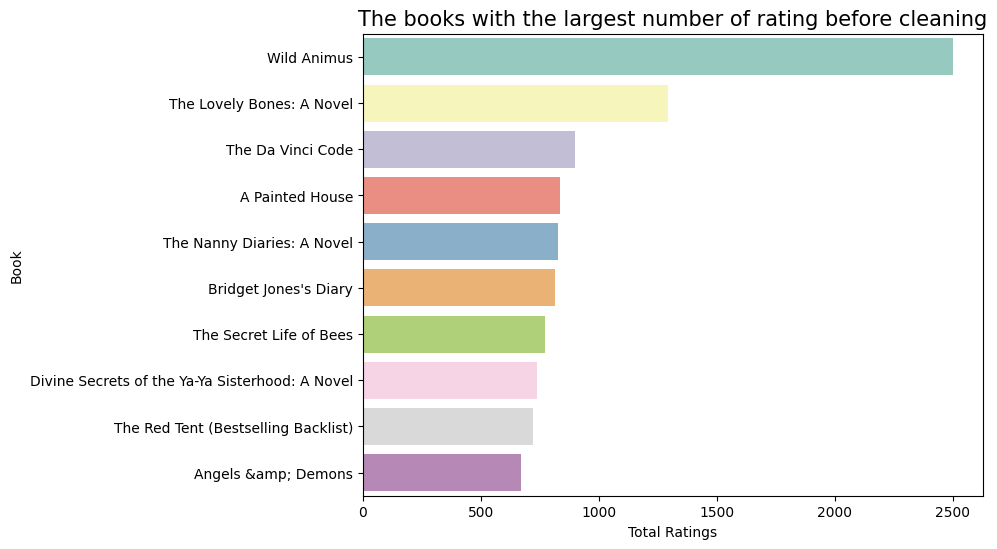
\includegraphics[width=1\linewidth]{img/Graphics/before_cleaning.png}
        \caption{Before Cleaning}
        \label{Before Cleaning}
    \end{figure}

    \begin{figure}[h]
        \centering
        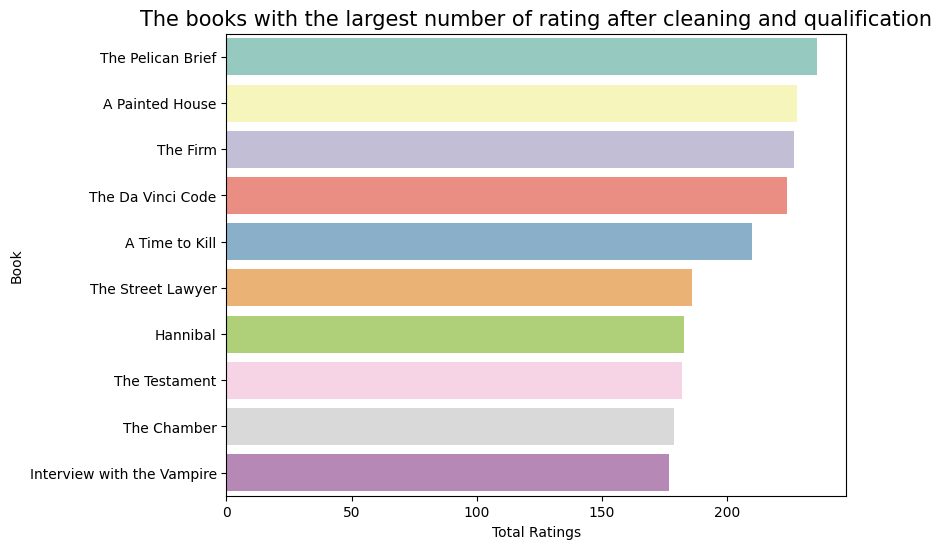
\includegraphics[width=1\linewidth]{img/Graphics/after-cleaning.png}
        \caption{After Cleaning}
        \label{After Cleaning}
    \end{figure}

    During data inspection, the notable outliers , influencing our data cleaning decisions has been identified to ensure a more accurate and representative data set.
     User IDs has been included for compatibility with the recommendation algorithm, facilitating seamless integration into the system.
     Ratings had exhibited a normal distribution, providing insights into the distribution of user preferences and guiding subsequent modeling decisions.
     \newpage
     The recommendation system developed using kNN, Matrix Factorization, Jaccard Similarity and Neural Network models achieved a relatively high recall of around 75\%, 95\%, 75\% and 86\% respectively, indicating identification of a large number of relevant items especially by kNN and MF model.
     However, most of the models boasted a modest precision of around 80\%, 55\%, 66\% and 57\% respectively indicating kNN model favoured popular items leading to more total relevant while Matrix Factorization model which relies on hidden pattern leading to lower precision. The recommendation system has been designed to encapsulate all models to strike a balance, providing both personalized and diverse suggestions. This approach aims to cater to individual user preferences while introducing novel items to enhance user exploration and satisfaction.
\begin{figure}[h]
        \centering
        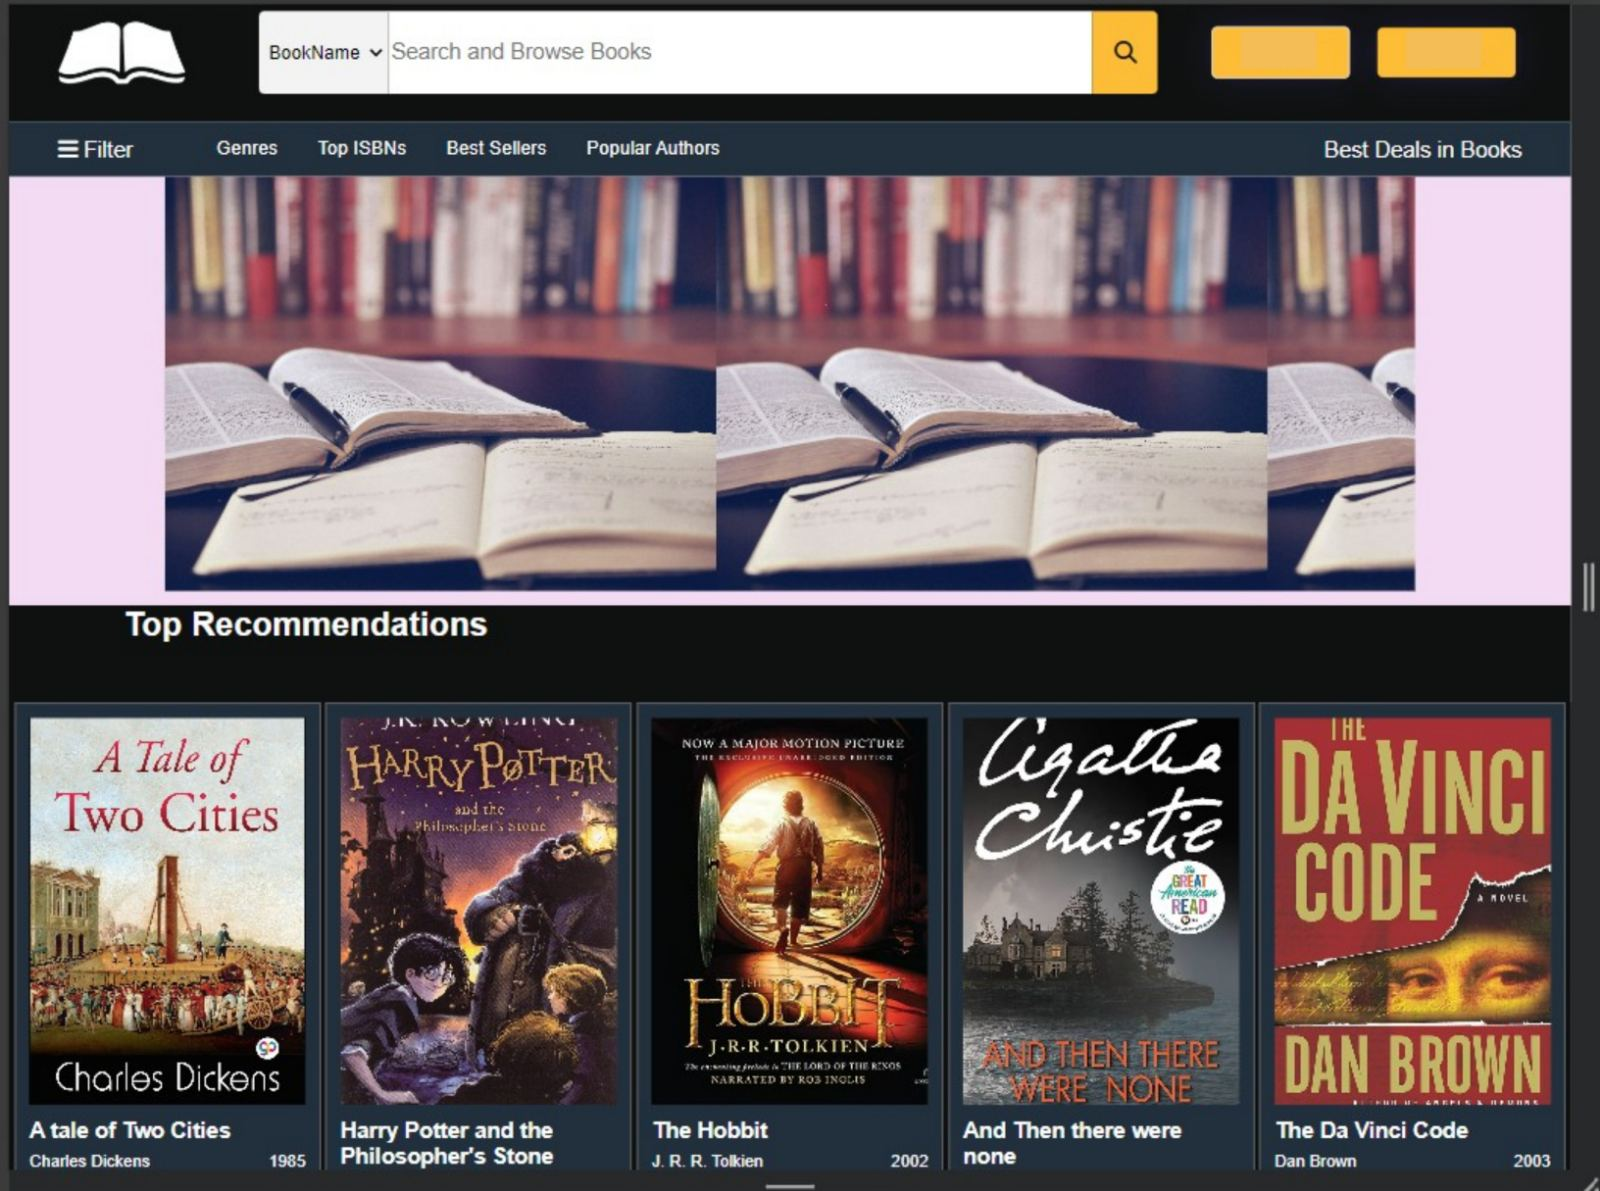
\includegraphics[width=0.8\linewidth]{img/Graphics/user interface.jpg}
        \caption{Home Page}
        \label{Home}
    \end{figure}
    
    The fig \ref{Home} shows the initial design of the UI of our web app. There is a search bar where you will get recommendations of the books similar to the books you wrote. There is also a top recommendations slide based on your current activity. There are options to see the top authors, top publisher and top rated books. This is only the initial design and final design may vary.

    \begin{figure}[h]
        \centering
        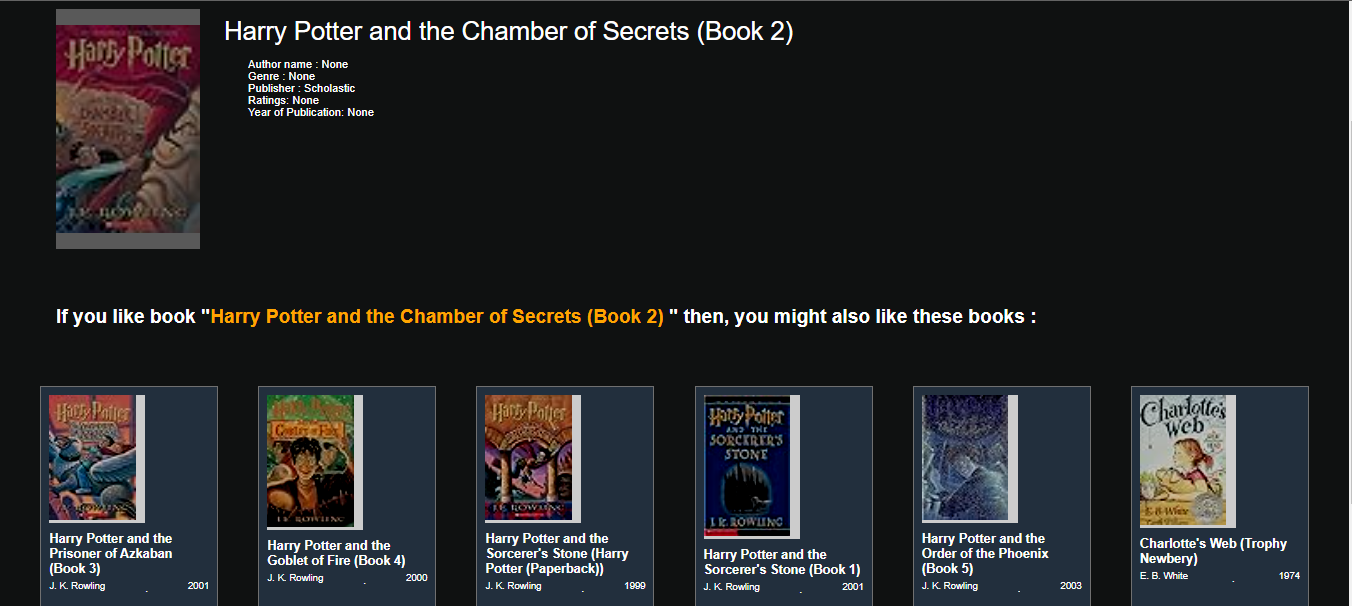
\includegraphics[width=0.9\linewidth]{img/Graphics/Secondpage.PNG}
        \caption{Second Page}
        \label{Secondpage}
    \end{figure}
    \newpage
    The fig \ref{Secondpage} shows the design of the secondpage UI of our web app. There is the details of the searched book along with 6 other books  with the recommended books author and year of publication.
    
    \newpage

    In the figures below showing metrics for recommendations comparison, blue line indicates the Precision, yellow line indicates Recall and the green line indicates the F1-score.

    The figure \ref{Metrics-knn-google} below shows the performance of kNN model against the recommendations collected through the google's recommendation engine. On some points lower values of metrics can be seen which can be attributed to the scarcity of supporting data. On some points such as book 0 and book 5 higher values of metrics can be seen which is due to the abundance of supporting data around it. The lower values of metrics can also be attributed to the preference of kNN model towards popular items.
    
    \begin{figure}[h]
        \centering
        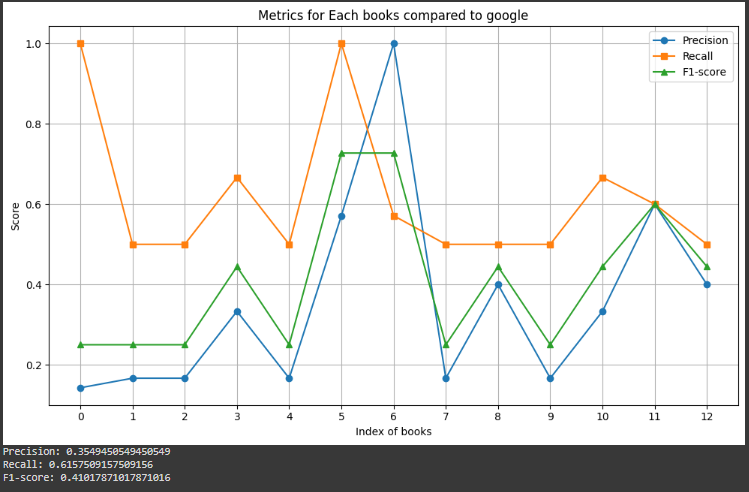
\includegraphics[width=1\linewidth]{img/Graphics/knn_google.PNG}
        \caption{Metrics of books compared to google using kNN model}
        \label{Metrics-knn-google}
    \end{figure}
    \newpage

    The figure \ref{Metrics-knn-amazon} shown below shows the performance of the kNN model compared to the recommendations collected via the amazon recommendation engine. A similar trend as visualized with the google recommendation engine can be seen.

    \begin{figure}[h]
        \centering
        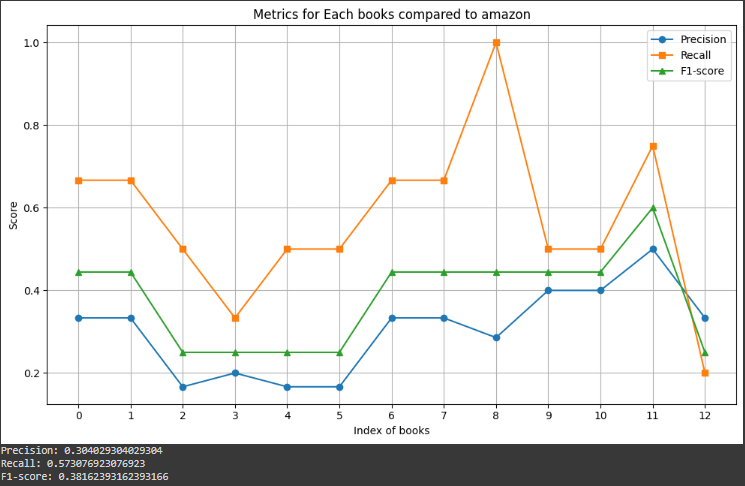
\includegraphics[width=1\linewidth]{img/Graphics/knn_amazon.PNG}
        \caption{Metrics of books compared to amazon using kNN model}
        \label{Metrics-knn-amazon}
    \end{figure}

    The figure \ref{Metrics-knn} shows the average ratings of books collected from both google and amazon. A good Recall can be seen which proves that the model is effective in recommending relevant items most of the times. Lower values of Precision and F1-score are due to data sparsity in the dataset and the smaller size of the dataset being compared to the enormous data access that google and amazon have. There are limited ratings for many books making it challenging for the model to accurately assess their relevance to users. Consequently, the precision of the model suffers as it struggles to distinguish truly relevant items from those that are less so.

    \begin{figure}[h]
        \centering
        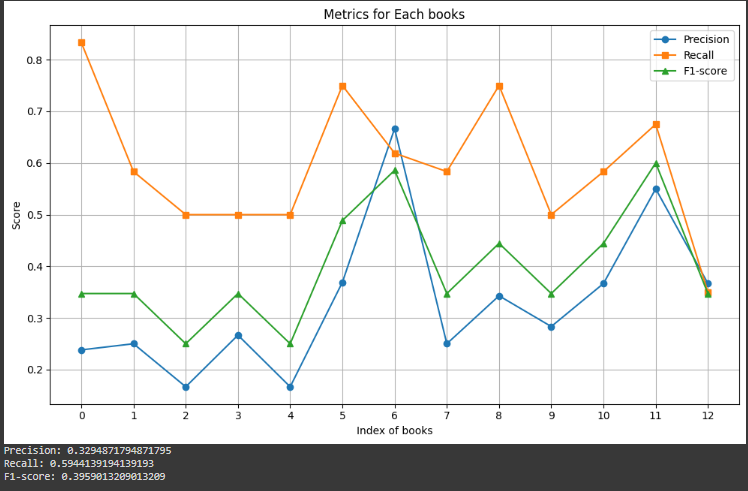
\includegraphics[width=1\linewidth]{img/Graphics/knn_model.PNG}
        \caption{Average metrics of books using kNN model}
        \label{Metrics-knn}
    \end{figure}
    \newpage

    The figure \ref{Metrics-mf-google} shown below show the performance of the Matrix Factorization model compared to the recommendations collected from google's recommendation engine. Though it handles data sparsity well, it was found that due to the amount of data fed into it, it was unable to determine latent factors effectively which consequently degraded it's values for Precision, Recall and F1-score.

    \begin{figure}[h]
        \centering
        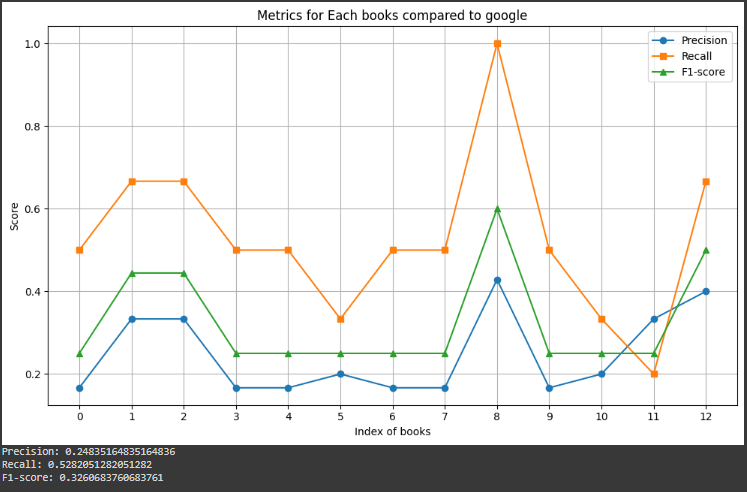
\includegraphics[width=1\linewidth]{img/Graphics/MF_model_google.PNG}
        \caption{Metrics of books compared to google using MF model}
        \label{Metrics-mf-google}
    \end{figure}
    \newpage

    The figure \ref{Metrics-mf-amazon} shown below shows the performance of the Matrix Factorization model compared to the recommendations collected from the amazon recommendation engine. Here, it is seen that the values for Precision, Recall and F1-score are quite average in all which might be because of our models similarity to amazon as our dataset has also been collected from amazon and kaggle.

    \begin{figure}[h]
        \centering
        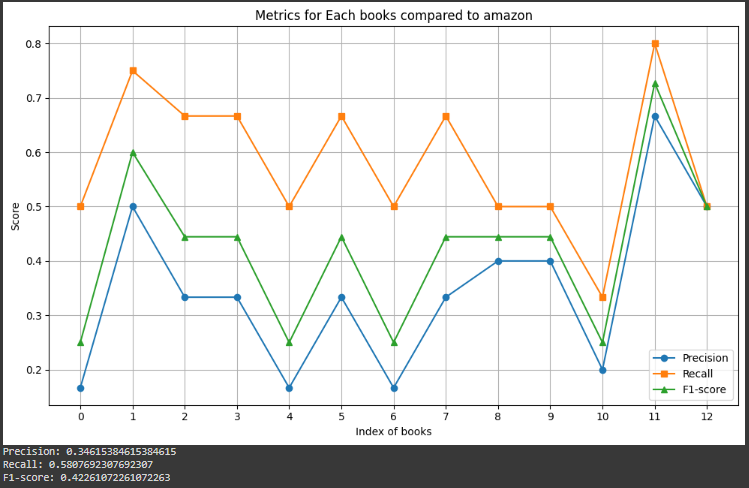
\includegraphics[width=1\linewidth]{img/Graphics/MF_model_amazon.PNG}
        \caption{Metrics of books compared to amazon using MF model}
        \label{Metrics-mf-amazon}
    \end{figure}

    \newpage

    The figure \ref{Metrics-mf} shows the average ratings of the Matrix Factorization model while comparing it to the recommendations gathered from both the google and the amazon recommendation engine. All in all, it shows a good recall with average values of Precision and F1-score.

    \begin{figure}[h]
        \centering
        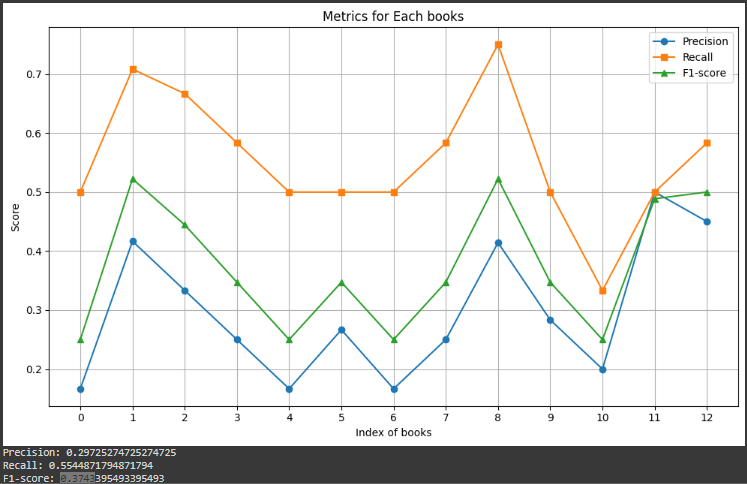
\includegraphics[width=1\linewidth]{img/Graphics/MF_model.PNG}
        \caption{Average metrics of books using MF model}
        \label{Metrics-mf}
    \end{figure}
    
    \newpage

    \begin{figure}[h]
        \centering
        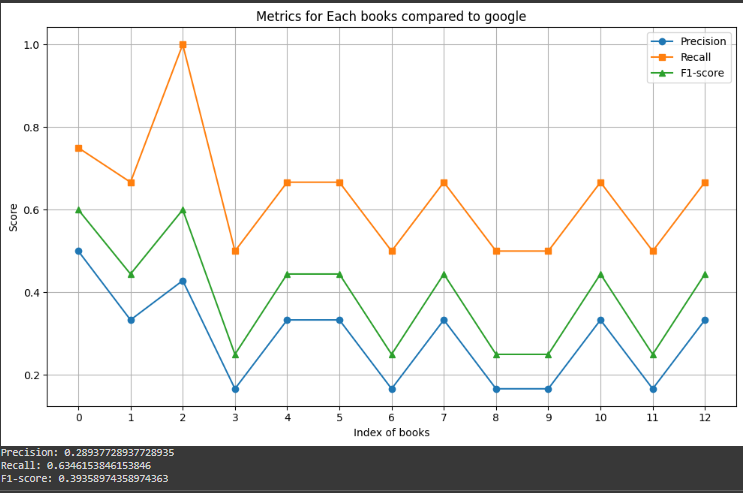
\includegraphics[width=1\linewidth]{img/Graphics/JS_Google.PNG}
        \caption{Average metrics of books using Jaccard Similarity model}
        \label{Metrics-js-google}
    \end{figure}

    The figure \ref{Metrics-js-google} shown below show the performance of the Jaccard Similarity model compared to the recommendations collected from google's recommendation engine. As, it treats all items equally and doesn't take into account the ratings or preferences of users for individual items which consequently degraded it's values for Precision, Recall and F1-score.
    
    \newpage

    \begin{figure}[h]
        \centering
        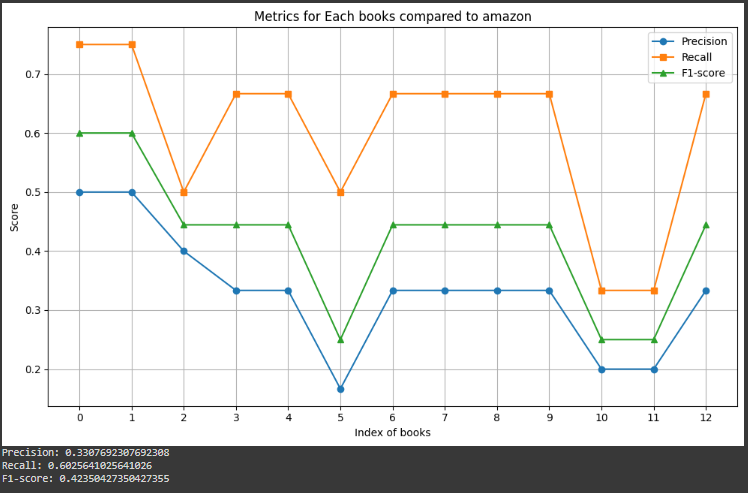
\includegraphics[width=1\linewidth]{img/Graphics/JS_Amazon.PNG}
        \caption{Average metrics of books using Jaccard Similarity model}
        \label{Metrics-js-amazon}
    \end{figure}

\newpage
    The figure \ref{Metrics-js-amazon} shown below shows the performance of the Matrix Factorization model compared to the recommendations collected from the amazon recommendation engine. Here, it is seen that the values for Precision, Recall and F1-score are bit higher in average which might be because of our models similarity to amazon as our dataset has also been collected from amazon and kaggle.
    
    \newpage

    \begin{figure}[h]
        \centering
        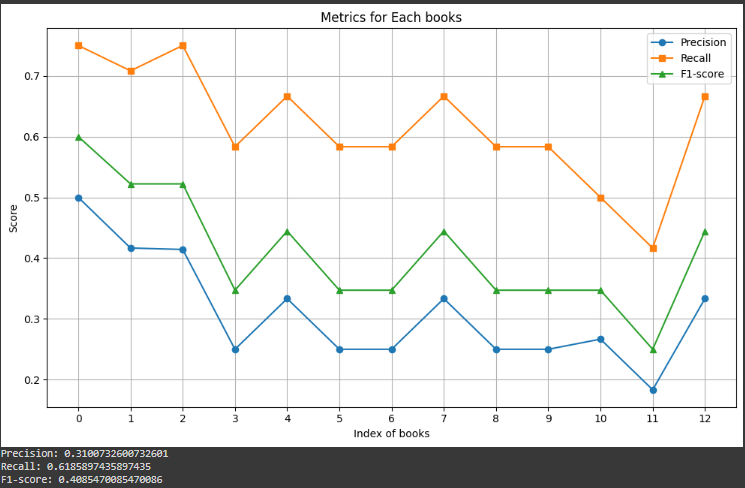
\includegraphics[width=1\linewidth]{img/Graphics/JS.PNG}
        \caption{Average metrics of books using Jaccard Similarity model}
        \label{Metrics-js}
    \end{figure}

    The figure \ref{Metrics-js} shows the average ratings of the Matrix Factorization model while comparing it to the recommendations gathered from both the google and the amazon recommendation engine. All in all, it shows a good recall with average values of Precision and F1-score i.e. pretty similar to kNN model as both methods rely on a similarity measure between the items.

    \newpage

    
The models were further evaluated by comparing them to each other. For this the pre-processed dataset was first split into train and test sets. On checking, train set had a record of 39308 books and the train set had a record of 9828 books. The same train set was used to train all four models and the same test set was used to validate the models. The threshold for confusion matrix of each model has been set to 0.15 which is a cutoff point for the probability or confidence level at which the model's predictions are considered as either positive or negative. Predictions with probabilities below this threshold are considered uncertain and may be treated differently, such as being classified as "uncertain" or requiring further evaluation. Once kNN, SVD and Jaccard models had generated their recommendations, they were compared against each other.

By visualizing the embeddings, an understanding can be gained on how the DNN represents the features of the items or users in a lower-dimensional space.

\begin{figure}[h]
        \centering
        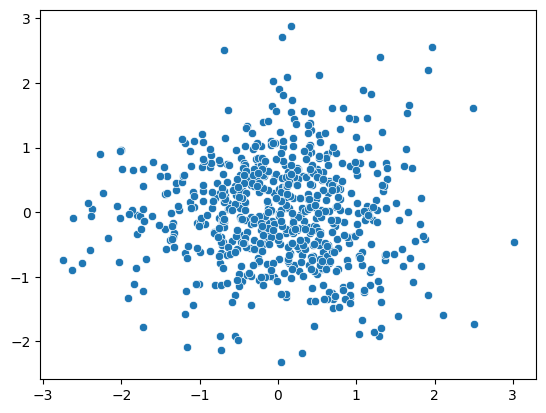
\includegraphics[width=1\linewidth]{img/Graphics/embeddings.png}
        \caption{Visualizing Embeddings for Neural Network}
        \label{embeddings}
    \end{figure}
    \newpage

The distance between embeddings in the visualized space reflects the semantic similarity between users. Users that are closer together in the embedding space are likely to have similar characteristics or preferences, while those farther apart may be more dissimilar. The points in the scatter plot \ref{embeddings} are exhibiting a pattern that is clustered together meaning that the model has been able to find meaningful relationships between the data.

The recommendations from the Neural Network were discreetized and the following ROC curve was drawn.

\begin{figure}[h]
        \centering
        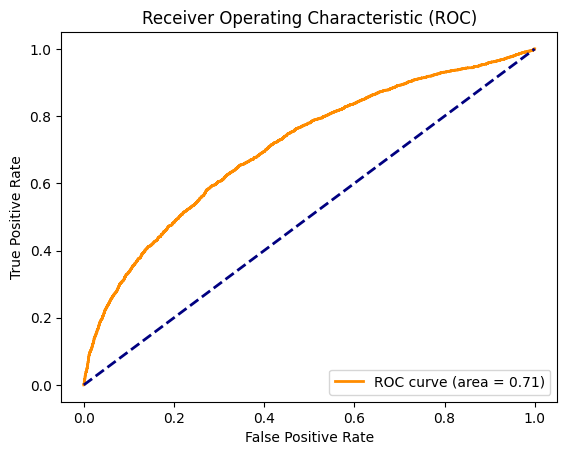
\includegraphics[width=1\linewidth]{img/Graphics/roc_nn.png}
        \caption{ROC Curve for Neural Network}
        \label{roc-nn}
    \end{figure}

    \newpage
It can be seen in the figure \ref{roc-nn} that AUC obtained is 0.71. The AUC of a ROC curve is a metric that quantifies the overall performance of the model. A higher AUC indicates that the model has better discriminative power, meaning it can effectively distinguish between the positive and negative classes. AUC of 0.71 means that there is an 71\% chance that the model will rank a randomly chosen positive instance higher than a randomly chosen negative instance. It means that if a positive instance i.e. a book that one will like and a negative instance i.e. a book that one will not like is picked randomly, then the model assigns higher probability to the positive instance 71\% of the time.

For the visualization of confusion matrix, true positives are placed on the top left corner, false positives on the top right corner, false negatives on the bottom left and true negatives on the bottom right corner.

\begin{figure}[h]
        \centering
        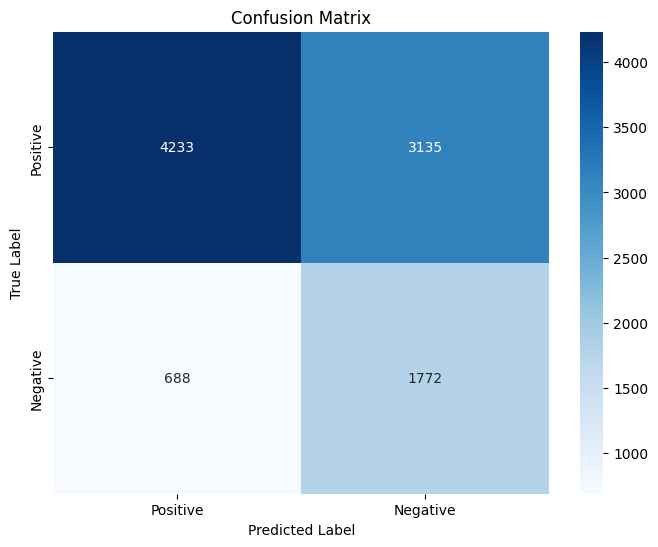
\includegraphics[width=1\linewidth]{img/Graphics/conf-nn.png}
        \caption{Visualizing Confusion Matrix for Neural Network}
        \label{conf-nn}
    \end{figure}

    \newpage

The figure \ref{conf-nn} shows that the model was correctly able to identify 4233 books as it is the number of true positives. Alongside, there were 3135 false positives, 688 false negatives and 1772 true negatives from the recommendation that the Neural Network provided. Through this, the evaluation metrics were calculated and found to be: precision of 0.5745, recall of 0.8601 and f1-score of 0.6889.

\begin{figure}[h]
        \centering
        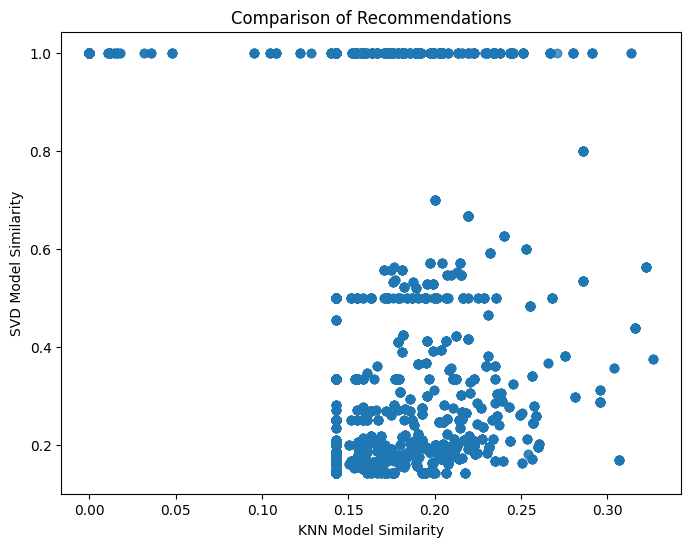
\includegraphics[width=1\linewidth]{img/Graphics/sim-plot.png}
        \caption{Visualizing the similarity of kNN and SVD}
        \label{sim-plot}
    \end{figure}

    \newpage

The figure \ref{sim-plot} shows how similar the recommendations from the kNN and SVD models are. The points very close to or at 1 mean that the recommendations provided by the kNN model and the SVD model are pretty similar while the points very close to 0 mean that the recommendations provided by the models are very different.

\begin{figure}[h]
        \centering
        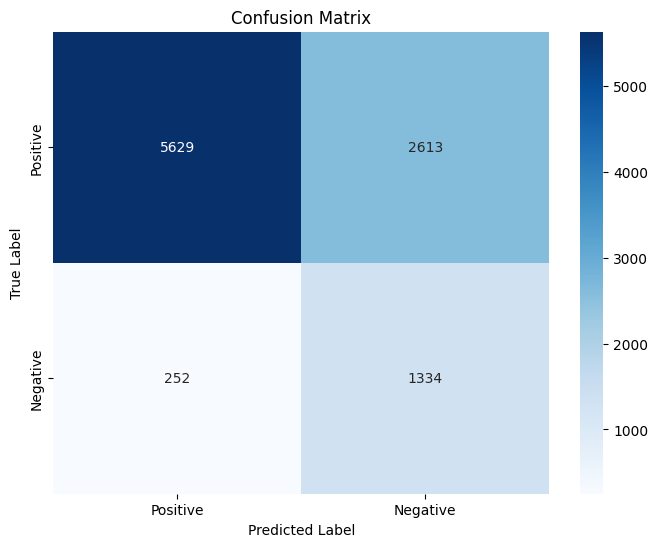
\includegraphics[width=1\linewidth]{img/Graphics/conf-knn-svd.png}
        \caption{Confusion Matrix after Comparing kNN and SVD}
        \label{conf-knn-svd}
    \end{figure}

    \newpage

The figure \ref{conf-knn-svd} shows the confusion matrix after comparing the kNN and SVD models. There were 5629 true positives, 2613 false positives, 252 false negatives and 1334 true negatives. The evaluations metrics calculated from this data were, precision of 0.6829, recall of 0.9572 and f1-score of 0.7971.

\begin{figure}[h]
        \centering
        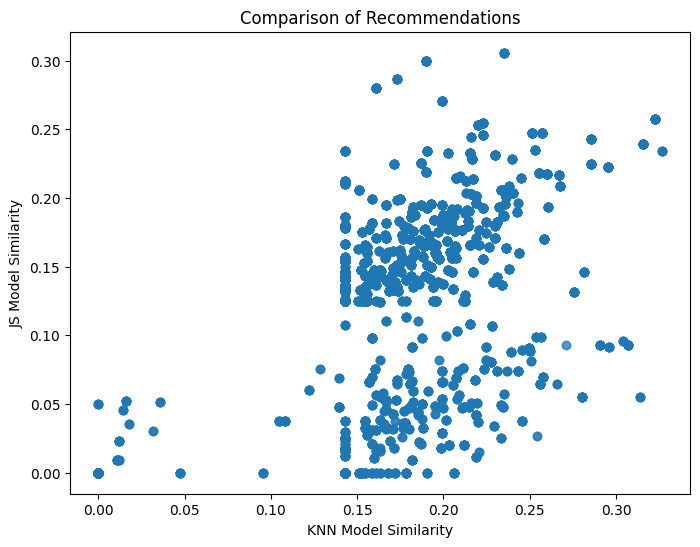
\includegraphics[width=1\linewidth]{img/Graphics/sim-knn-js.png}
        \caption{Visualizing the Similarity of kNN and Jaccard}
        \label{sim-knn-js}
    \end{figure}

    \newpage

The figure \ref{sim-knn-js} shows that the recommendations provided by kNN and Jaccard are not very similar to each other as the points are well within the range of 0.3.


\begin{figure}[h]
        \centering
        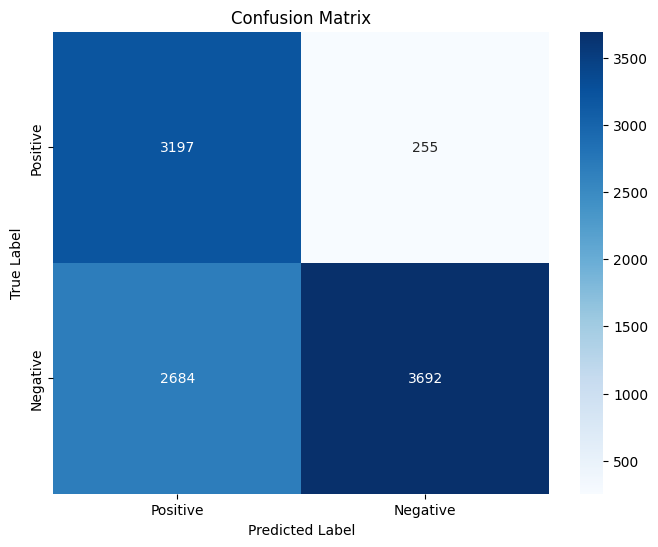
\includegraphics[width=1\linewidth]{img/Graphics/conf-knn-js.png}
        \caption{Confusion Matrix after Comparing kNN and Jaccard}
        \label{conf-knn-js}
    \end{figure}

    \newpage

The figure \ref{conf-knn-js} shows that 3197 true positives, 255 false positives, 2634 false negatives and 3692 true negatives were identified. Through this, the precision was found to be 0.9261, recall was 0.5436 and the f1-score was 0.6850.

\begin{figure}[h]
        \centering
        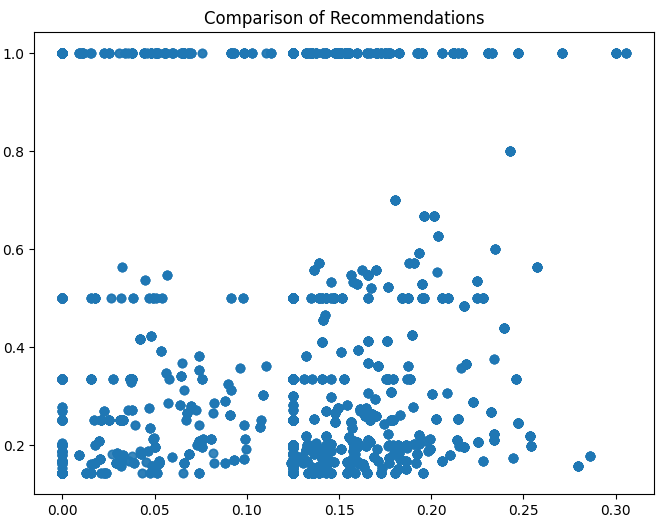
\includegraphics[width=1\linewidth]{img/Graphics/sim-js-svd.png}
        \caption{Visualizing the similarity of SVD and Jaccard}
        \label{sim-js-svd}
    \end{figure}

    \newpage
    
In the scatter plot SVD similarities are placed in the y-axis and the Jaccard similarities in the X-axis.The points close to 1 in the scatter plot \ref{sim-js-svd} show that the recommendations provided by the two models are somewhat similar.

\begin{figure}[h]
        \centering
        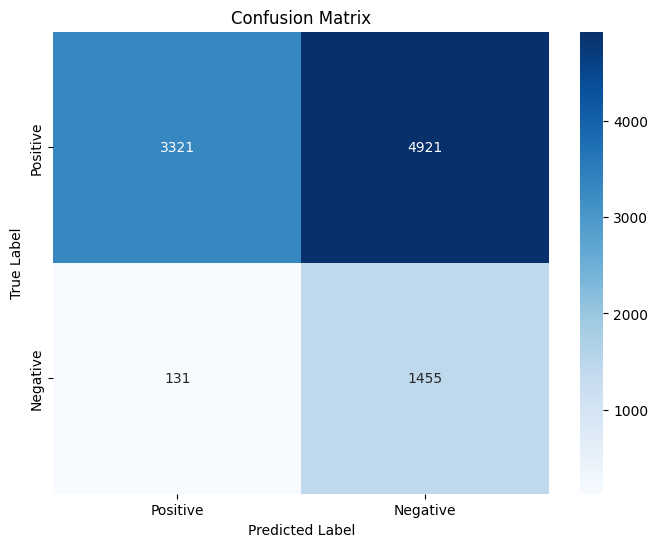
\includegraphics[width=1\linewidth]{img/Graphics/conf-js-svd.png}
        \caption{Confusion Matrix after Comparing SVD and Jaccard}
        \label{conf-js-svd}
    \end{figure}

    \newpage

The figure \ref{conf-js-svd} shows that 3321 true positives, 4921 false positives, 131 false negatives and 1455 true negatives were identified. From these values, the calculated precision was 0.4029, recall was 0.9620 and f1-score was 0.5679.   

 Four commonly used algorithms have been trained and compared to each other. The performance of these models were evaluated based on precision, recall and F1-score.

The kNN model had a precision of 0.8045, recall of 0.7503, and F1-score of 0.7410. The Matrix Factorization model had a precision of 0.5429, recall of 0.9595, and F1-score of 0.6825. Jaccard's Similarity had a precision of 0.6645, recall of 0.7528 and a F1-score of 0.6264. The Neural Network had a precision of 0.5745, recall of 0.8601 and F1-score of 0.6889. From the given metrics, it can be inferenced that the kNN model is better than the other models with the best precision of all the models and overall balanced recall and F1-score.

The best case theoretical output had been set at precision, recall and F1-score of around 0.7. In this context, the models have exceeded the expectations after fine 
tuning their parameters. The kNN model has every parameter above the initially set values. Matrix Factorization model though falls back in precision, it's recall was found to be highly impressive given it's capability to handle sparse datasets well. Jaccard's Similarity showed similar metrices to that of the Neural Network with comparable values for the provided threshold. Jaccard's Similarity had higher precision while Neural Network had higher recall.

The performance of our models has also been evaluated in the context of their strengths and weaknesses. The kNN model, while simple and easy to implement, tends to identify a large number of relevant items mostly popular items and might struggle to recommend users with unique tastes. On the other hand, the Matrix Factorization model, while more complex, could uncover latent factors that  captures underlying structures in the dataset and provide more personalized recommendations. Additionally, handling missing values and incorporating side information (e.g. user demographics, book attributes) can further improve the accuracy of recommendations. Jaccard's Similarity and Neural Network seem to work well when there are larger sets of data to be trained with showing capable relationship determining abilities but seemed lacking for the amount of data that was fed into the model. Moving forward, potential research explore hybrid approaches that encompasses the strengths of both models for further improved recommendation performance.
